\documentclass[11pt]{article}
\usepackage{mathpazo}
\usepackage{url}
\usepackage{graphicx}
\usepackage{verbatim}

\newcommand{\eri}{\textsc{Erigone}}
\newcommand{\prm}{\textsc{Promela}}
\newcommand{\eui}{\textsc{EUI}}
\newcommand{\p}[1]{\texttt{#1}}
\newcommand{\bu}[1]{\textsf{#1}}

\textwidth=15cm
\textheight=22cm
\topmargin=0pt
\headheight=0pt
\oddsidemargin=1cm
\headsep=0pt
\renewcommand{\baselinestretch}{1.1}
\setlength{\parskip}{0.20\baselineskip plus 1pt minus 1pt}
\parindent=0pt

\title{The \eui{} Development Environment for the\\
\eri{} Model Checker\\User's Guide and Software Documentation\\
\mbox{}\\\large{Version 1.8.4}}       % Change version number
\author{Mordechai (Moti) Ben-Ari\\
Department of Science Teaching\\
Weizmann Institute of Science\\
Rehovot 76100 Israel\\
\textsf{http://stwww.weizmann.ac.il/g-cs/benari/}}
%\date{}
\begin{document}
\maketitle
\thispagestyle{empty}

\vfill

\begin{center}
Copyright \copyright{} 2009-12 by Mordechai (Moti) Ben-Ari.
\end{center}

This work is licensed under the Creative Commons Attribution-ShareAlike 3.0
License. To view a copy of this license, visit
\url{http://creativecommons.org/licenses/by-sa/3.0/}; or, (b) send a letter
to Creative Commons, 543 Howard Street, 5th Floor, San Francisco,
California, 94105, USA.

\newpage

\section{Introduction}

\eui{} is a graphical user interface for the \eri{} Model Checker that
is used for simulating and verifying concurrent programs. It is an
adaptation of the \textsc{jSpin} interface for \textsc{Spin}. The user
interface of \eui{} is simple, consisting of a single window with menus,
a toolbar and three adjustable text areas. \eri{} option strings are
automatically supplied and the \eri{} output is filtered and formatted.
All aspects of \eui{} are configurable: some at compile time, some at
initialization through a configuration file and some at runtime.

\subsection*{References}
\begin{itemize}
\item M. Ben-Ari. \textit{Principles of the Spin Model Checker}. Springer, 2008.
\item M. Ben-Ari. \textit{The \eri{} Model Checker}. \url{http://code.google.com/p/erigone/}.
\end{itemize}

\section{Installation and execution}

\subsection{Installation}

\begin{quote}
The following description is for Windows. For other systems, download
and open the \eui{} zip file and then copy \eri{} executable to the
\eui{} directory.
\end{quote}

Install the Java SDK or JRE (\url{http://java.sun.com}).\footnote{The
default font for \eui{} is \p{Lucida Sans Typewriter}. This font may no longer be
available in the JRE you use. If you have the fonts from a previous version you
can copy them to the \p{lib/fonts} directory as explained in
\url{http://java.sun.com/j2se/1.5.0/docs/guide/intl/font.html}. Alternatively,
you can change the configuration file to use a monospaced font such as
\p{Courier} that is installed by default.} \eui{} needs Java 1.5 at least.

Download the \eui{} installation file called \p{eui-N.exe},
where \p{N} is the version number, and execute the installation file.
The installation will create the following subdirectories: \p{docs} for
the documentation, \p{eui} for the source files, \p{txts} for the text
files (help, about and copyright), and \p{examples}.

\subsection{Execution}

To run \eui{}, execute the command \p{javaw -jar EUI.jar}.
An optional argument names the \prm{} file to be opened initially.

By default, an icon to run \eui{} is installed on the Windows Desktop.
If Java is associated with \p{jar} files, double-clicking on the icon
will run \eui{}.


\subsection{Configuration}

Configuration data (Appendix~\ref{a.cfg}) is in the file \p{config.cfg}.
\textbf{When upgrading \eui{}, erase the configuration file before
installing a new version, so that new configuration options will be
recognized.} \eui{} searches for the configuration file in the current
directory; if it is not found, \eui{} searches for it in the directory
where the jar file is installed; if it is not found there, a new file
with default values is written.

\subsection{Building}

To build \eui{}, run:
\vspace{-1em}
\begin{verbatim}
         javac -target 1.5 eui\*.java
         jar cfm EUI.jar eui\MANIFEST.MF eui\*.class
\end{verbatim}
\vspace{-2em}

\section{\eui{} user interface}
The user interface includes a menu, a toolbar and three text areas.
Menu and toolbar commands have keyboard mnemonics or accelerators.
These can be easily configured by modifying the file \p{Config.java} and
rebuilding.

The left text area is used to display \prm{} source files. The bottom
text area is used to display messages from both \eri{} and \eui{}. The
right text area is used to display the output from \eri{}: statements
executed, values of variables and results of verifications. The text
areas can be resized by dragging the dividers and an area can be hidden
by clicking on the triangles in the dividers; the initial sizes can be
set in the configuration file. The toolbar button \bu{Maximize}
(\bu{Alt-M}) toggles between a normal split pane and a maximized right
text area that displays the \eri{} output.

\begin{figure}[tb]
\begin{center}
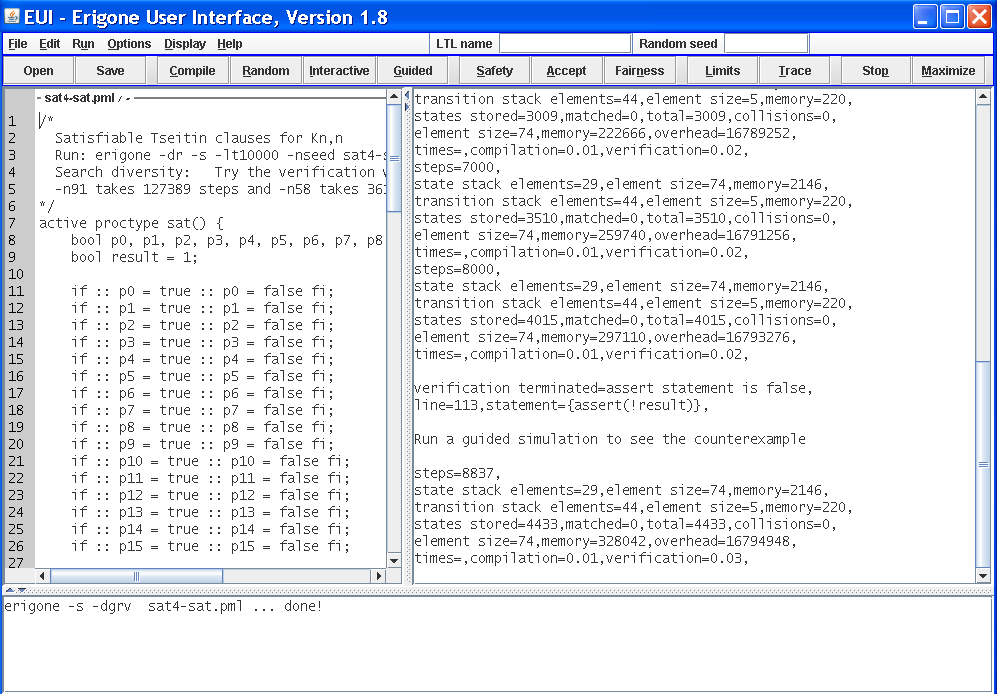
\includegraphics[width=140mm]{eui}
\end{center}
\end{figure}

\subsection{Menu items}

\begin{description}
\item[\bu{File}] This menu includes selections for \bu{New}, \bu{Open}, 
\bu{Save}, \bu{Save As}, and \bu{Exit}. \bu{Switch file} closes the 
current file and opens the last file that was edited, if any.

\item[\bu{Edit}] This menu includes selections for \bu{Undo}, \bu{Redo}, 
\bu{Copy}, \bu{Cut}, \bu{Paste}, \bu{Find} and \bu{Find again}.

\item[\bu{Run}] This menu replicates the buttons on the toolbar for
running \eri{} in various modes. See the description in the next
section.

\item[\bu{Options}] The following \eri{} \bu{Limits} can be set (the
values are in thousands):
\begin{itemize}
\item \bu{Total steps}: The total number of steps in an execution of
\eri{}.
\item \bu{Progress steps}: A progress message will be displayed
after this number of steps of a verification.
\item \bu{State stack}, \bu{Location stack}: The size of the
verification stacks.
\end{itemize}

\bu{Default} restores the default values and \bu{Save} saves the current
options in the configuration file, together with the last directory from
which a source file was opened, and the current values of the splitpane
dividers. The file can be saved to the \bu{current} or \bu{install}
directory.

\item[\bu{Display}] This menu controls the display of the output in the
right text area.
\begin{itemize}
\item \bu{Maximize} replicates the button on the toolbar.
\item \bu{Save output} saves the contents of the text area in a file with
extension \p{.out}.
\item The \bu{Trace} submenu is discussed in
Section~\ref{s.run}.
\end{itemize}

\item[\bu{Help}] \bu{Help} displays a short help file and \bu{About} 
displays copyright information.
\end{description}

\subsection{Textfields in the menu bar}

The field \bu{LTL name} is used to select a named LTL (inline)
specification as described in Section~\ref{s.ltlname}.

A numeric (non-blank) value in the field \bu{Random seed} will be used as the
seed for generating random numbers, enabling a random simulation to be
repeated. During verification it is used for search diversity. See the
\eri{} User's Guide for details.

\newpage

\section{Running \eri{}}\label{s.run}
In the \bu{Run} menu and on the toolbar are eight selections for
running \eri{}. They all use the \prm{} source file that has been opened,
and save the file before execution.
During simulation and verification,
you can select \bu{Stop} to terminate the \eri{} process that has been forked.
\begin{description}
\item[\bu{Comple}] Runs the \prm{} compiler.
\item[\bu{Random}] Runs a random simulation.
\item[\bu{Interactive}] Runs an interactive simulation.
\item[\bu{Guided}] Runs a guided simulation using the trail
file created for a counterexample found in a verification.
\item[\bu{Safety}] Runs a safety verification.
\item[\bu{Accept}] Runs an acceptance verification.
\item[\bu{Fairness}] Runs an acceptance verification with weak fairness.
\end{description}

\textbf{If you terminate \eui{} while \eri{} is running (for example by
entering \bu{ctrl-C} at the command line), make sure to terminate the
\eri{} process as well.} In Windows, press \bu{ctrl-alt-del}, \bu{Task
List} and \bu{Processes}. Select \bu{erigone.exe} and \bu{End Process}.

\subsection{Simulation}\label{s.sim}

\subsubsection{Interactive simulation}

During an interactive simulation, if there is more than one executable
statement or expression in a state, a dialog frame will pop up with the
current values of the variables and a list of the statements and
expressions that can be executed. The list can be displayed either as a
row of buttons, or---if there is not enough room---as a pulldown menu.
The choice of the format is determined by the value of the configuration
option \p{SELECT\_MENU}. There are also configuration options for
setting the width and height of the buttons or menu items.

The dialog can be navigated using the mouse; closing the dialog frame
will terminate interactive simulation. For keyboard navigation:
\begin{description}
\item[Buttons] \bu{Tab} and \bu{Shift-Tab} move through the buttons
and \bu{Space} selects the highlighted button. Press \bu{Esc} to terminate.
\item[Menu] Press the \bu{Down arrow} to display the list and to highlight the
item you want; press \bu{Return} to select it. Press \bu{Esc} to terminate.
\end{description}

\subsubsection{Filtered output}\label{s.filter}
The contents of the \eri{} output can be changed by selecting 
\bu{Display/Trace}. This pops up a dialog that can be used to set the
width of the field for the statement executed and the width of the field
for each variable. There are text areas for entering a list of strings defining 
variables to be \emph{excluded} from the display. Any variable containing 
a string from the list is not displayed; for example, \p{want} will 
exclude all variables that have \p{want} as a substring. If the variable name is 
prefixed by \p{+}, it will be included anyway. For example, if you have an 
array variable \p{test}, then the entries \p{test} and \p{+[1]} will 
exclude display of the elements of \p{test} except for \p{test[1]}. The 
list is saved in a file with extension \p{.exc}.

Similarly, a file of excluded statements can be created; a statement is
excluded if it contains one of the substrings in the file. The same
convention for the prefix \p{+} enables inclusions of strings that would
otherwise be excluded. The file extension is \p{.exs}. \bu{Exclude
statements} should \emph{not} be used with interactive simulation.

When a non-active \p{proctype} is used, the local variables such as
\p{P.temp} are only formal names. When \p{run} creates a process, actual
variables names \p{P\_1.temp}, \p{P\_2.temp}, \ldots{} are created and
the formal variable is removed from the display.

\subsection{LTL formulas}\label{s.ltlname}
A correctness claim is specified by a formula
in \emph{Linear Temporal Logic (LTL)}. The formula is written inline
within the program:\footnote{\eri{} supports specifying LTL formulas in
an external file, but this is not supported in \eui{}.}
\begin{verbatim}
ltl { [](critical <= 1) }
\end{verbatim}
If there are named LTL formulas within the program:
\begin{verbatim}
ltl mutex { []!(csp && csq) }
ltl nostarve { []<>csp && []<>csq }
\end{verbatim}
you can enter the name of the formula to be used in the field \bu{LTL
name}.

\eri{} requires a LTL formula for verification of \emph{acceptance}
(with or without fairness). A formula is optional for verifying safety;
if a formula is not needed, be sure to erase any data in the LTL field.

\newpage

\section{Software structure}

\p{EUI} is the main class and contains declarations of the GUI
components and instances of the classes \p{Editor} and \p{RunSpin}.
Method \p{init} and the methods it calls initialize the GUI. Method
\p{action\-Per\-formed} is the event handler for all the menu items and
buttons; it calls the appropriate methods for handling each event. The
\bu{About} and \bu{Help} options are implemented by reading files
\p{copyright.txt} and \p{help.txt}, respectively, and displaying them in
the righthand pane.

\p{Filter} performs the filtering of the \eri{} output. Since it is
called for each line separately there are quite a number of flags to
maintain state between lines. \p{ArrayList}s are used to store the
excluded variables and statements, while \p{variables} of type
\p{TreeMap} is used to map variable names into values. Whenever a state
is displayed in the output (for example, \p{"temp=6,"},
\p{storeVariables} is called to search for the line for each key in the
map and set the value associated with the name. \p{variablesToString}
iterates over the map to create a string of the values of the variables,
while \p{collectionToString} creates the title lines with the variable
names. The actual processing of the output is performed in three
separate methods, one for compilation, one for simulation and one for
verification.

\p{EUIFileFilter} is used with a \p{JFileChooser} when opening and
saving files: \prm{} source files, LTL property files and \eri{} save
output files.

\p{Limits} is the dialog frame for \bu{Options/Limits} and \p{Trace} is
the dialog frame for editing the list of variable strings to be excluded
from the display.

\p{Config} contains declarations of compile time configuration items.
Method \p{init} calls \p{set\-Default\-Properties} to initialize the
instance of \p{Properties} with the default values of the dynamic
configuration items; it then attempts to load the configuration file,
and if unsuccessful, the default properties are written to a new file.

\p{Editor} implements an editor using operations on a \p{JTextArea}. It
implements the interface \p{Document\-Listener} to flag when the source
has been modified. The class is also responsible for the LTL formula
\p{JTextField}. \p{EUI} calls method \p{writeFile} to write \p{out}
files, and method \p{readFile} to read the text files to be displayed.

\p{LineNumbers} extends a \p{JComponent} to create line numbers for the
\p{RowHeaderView} of the editor \p{JScrollPane} (thanks to Niko Myller
for this code).

\p{UndoRedo} was extracted from an example on the Java web site.

The event handler in \p{EUI} calls \p{run} in class \p{RunSpin} to
execute \eri{}. \p{run} creates a thread of class \p{RunThread}, and
uses \p{ProcessBuilder} to set up the command, directory, merge the
output and error streams, and set up streams for I/O. The call
\p{runAndWait} is used for short calls like \bu{Compile}; this call does
not return until the completion of the subprocess. The call \p{run} will
return immediately after it has created the thread. In this case, the
event handler in \p{EUI} calls \p{isSpinRunning} to create a thread to
poll for termination of \eri{}; by creating a separate thread, the event
handler is freed to accept a selection of \bu{Stop}.

When more than one executable transition occurs during an interactive
simulation, the method \p{select} is called. This method pops up a
dialog to enable the user to make a selection. A \p{JFrame} is created
in a new thread of the inner class \p{SelectDialog} to wait for the
selection. \p{select} polls \p{selectedValue} which is set with the
selected button value or zero if the frame is closed or \bu{Esc}
pressed. In that case, \p{q} is sent to \eri{} to terminate the
simulation.

\appendix

\section{Configuration file}\label{a.cfg}

These tables give the properties in the configuration file and their
default values.

\begin{center}

\begin{tabular}{|p{.3\textwidth}|p{.4\textwidth}|}
\hline
\multicolumn{2}{|c|}{Directories and files}\\ \hline
\textsc{\ttfamily SOURCE\_DIRECTORY} & \verb+examples+ \\
\textsc{\ttfamily ERIGONE} &\verb+erigone.exe+ \\
\textsc{\ttfamily HELP\_FILE\_NAME} &\verb+txt\help.txt+\\
\textsc{\ttfamily ABOUT\_FILE\_NAME} &\verb+txt\copyright.txt+\\
\hline
\end{tabular}

\bigskip

\begin{tabular}{|p{.3\textwidth}|p{.4\textwidth}|}
\hline
\multicolumn{2}{|c|}{Options for executing \eri{}}\\ \hline
\textsc{\ttfamily COMPILE\_OPTIONS} &\verb+-c -dbprv+\\
\textsc{\ttfamily RANDOM\_OPTIONS} &\verb+-r -dcmoprv+\\
\textsc{\ttfamily INTERACTIVE\_OPTIONS} &\verb+-i -dcemoprv+\\
\textsc{\ttfamily TRAIL\_OPTIONS} &\verb+-g -dcmoprv+\\
\textsc{\ttfamily SAFETY\_OPTIONS} &\verb+-s -dgrv+\\
\textsc{\ttfamily ACCEPT\_OPTIONS} &\verb+-a -t -dgrv+\\
\textsc{\ttfamily FAIRNESS\_OPTIONS} &\verb+-f -t -dgrv+\\
\hline\hline
\textsc{\ttfamily TOTAL\_STEPS} & \verb+100+\\
\textsc{\ttfamily PROGRESS\_STEPS} & \verb+1+\\
\textsc{\ttfamily STATE\_STACK} & \verb+2+\\
\textsc{\ttfamily LOCATION\_STACK} & \verb+3+\\
\textsc{\ttfamily SEED} & \verb+0+\\
\textsc{\ttfamily SINGLE\_QUOTE} & \verb+false+\\\hline
\end{tabular}

\bigskip

\begin{tabular}{|p{.3\textwidth}|p{.4\textwidth}|}
\hline
\multicolumn{2}{|c|}{Trace options}\\ \hline
\textsc{\ttfamily PROCESS\_WIDTH} & \verb+7+\\
\textsc{\ttfamily STATEMENT\_WIDTH} & \verb+18+\\
\textsc{\ttfamily VARIABLE\_WIDTH} &\verb+10+\\
\textsc{\ttfamily LINES\_PER\_TITLE} &\verb+20+\\
\hline
\end{tabular}

\bigskip

\begin{tabular}{|p{.3\textwidth}|p{.4\textwidth}|}
\hline
\multicolumn{2}{|c|}{Text settings}\\ \hline
\textsc{\ttfamily WRAP} &\verb+true+\\
\textsc{\ttfamily TAB\_SIZE} &\verb+4+\\
\textsc{\ttfamily FONT\_FAMILY} & \verb+Lucida Sans Typewriter+\\ 
\textsc{\ttfamily FONT\_STYLE} & \verb+java.awt.Font.PLAIN+\\
\textsc{\ttfamily FONT\_SIZE} & \verb+14+\\\hline
\end{tabular}

\bigskip

\begin{tabular}{|p{.3\textwidth}|p{.4\textwidth}|}
\hline
\multicolumn{2}{|c|}{Frame size}\\ \hline
\textsc{\ttfamily WIDTH} &\verb+1000+\\
\textsc{\ttfamily HEIGHT} &\verb+700+\\\hline
\end{tabular}

\bigskip

\begin{tabular}{|p{.3\textwidth}|p{.4\textwidth}|}
\hline
\multicolumn{2}{|c|}{Interactive dialog settings}\\ \hline
\textsc{\ttfamily SELECT\_BUTTON} &\verb+120+\\
\textsc{\ttfamily SELECT\_HEIGHT} &\verb+70+\\
\textsc{\ttfamily SELECT\_MENU} &\verb+5+\\\hline
\end{tabular}

\bigskip

\begin{tabular}{|p{.3\textwidth}|p{.4\textwidth}|}
\hline
\multicolumn{2}{|c|}{Location of dividers}\\ \hline
\textsc{\ttfamily LR\_DIVIDER} &\verb+400+\\
\textsc{\ttfamily TB\_DIVIDER} &\verb+500+\\
\textsc{\ttfamily MIN\_DIVIDER} &\verb+50+\\\hline
\end{tabular}

\bigskip

\begin{tabular}{|p{.3\textwidth}|p{.4\textwidth}|}
\hline
\multicolumn{2}{|c|}{Delay while waiting for user input}\\ \hline
\textsc{\ttfamily POLLING\_DELAY} &\verb+200+\\\hline
\end{tabular}

\bigskip

\begin{tabular}{|p{.3\textwidth}|p{.4\textwidth}|}
\hline
\multicolumn{2}{|c|}{Display \eri{} output that is piped to \eui{}}\\ \hline
\textsc{\ttfamily DEBUG} &\verb+false+\\\hline
\end{tabular}

\end{center}
\end{document}
